\chapter{Results}
\label{sec:results}

\newcommand\expone{\textbf{Yields}}
\newcommand\exptwo{\textbf{Yields+IMFslope}}
\newcommand\expthree{\textbf{Yields+IMFslope+NSM}}
There are three main experiments;
\begin{description}
\item[\expone] The yields of isotopes are varied within their standard deviation \comment{Add reference to arnould table}
\item[\exptwo] Same as \expone, with the high mass slope of the initial mass function, $\alpha$, varied within the uncertainty found in \mycite{cote16a}, which is $\sigma_{\alpha}=8.73\%$ around the mean $\langle \alpha \rangle = 2.29$.
\item[\expthree] Same as \exptwo, with a ten percent uncertainty in parameters related to neutron star mergers. These are the fraction of binary neutron stars that turn to neutron star mergers (scales the rate of neutron star mergers), the ejecta mass (scales the total mass ejected from a neutron star merger), and the slope of the delay-time distribution (distribution of time between neutron star formation and merger for a system that will merge).
\end{description}
It should be noted that the 10\% uncertainty in \expthree is rather arbitrary.
It is diffeicult to find realistic realizations of the probability distribution of the \textit{neutron star merger parameters} in \expthree, and the experiments is merely used to compare the effect of varying the astrophysical source.
%1500 sims
The experiments pick a randomly generated number (within the appropriate gaussian distribution) and calculates the chemical evolution with \omegamodel.
The calculations are performed 1500 times with randomly generated deviations to the parameters.
The number is also chosen rather arbitrarily, it is more than twice the amount of calculations for multiple parameters in \mycite{cote16a} and should be sufficient for the purpose of this thesis.

%present data
The solar system is formed from a collapse of interstellar gas.
The gas is assumed to have separated from the interstellar medium at the formation of the solar system.
The formation of the solar system is estimated from meteorites to be $\simeq$ 4.5 Gyrs ago \mycite{bouvier10}.
From the semianalytical model, \omegamodel, the total mass of \os{187} and \re{187} in the interstellar medium is calculated.
The cosmic clock fraction between the two isotopes, $f_{187} = \frac{\os{187}}{\re{187}}$, is also calculated.
The fraction between the isotopes is relevant because it can be determined from meteorites, unlike the total mass of isotopes in the \sos\ at the time of formation.
In the \eris-simulation the galactic age is 14 Gyrs, which means the solar system formed at 9.5 Gyrs.
The uncertainties of the mass of each isotope come from the uncertainty of the input parameters in each experiment, \expone, \exptwo, and \expthree.
The cosmic clock fraction, $f_{187}$, is determined from observations to be \comment{insert value+deviation here}, see table \ref{tab:obs-cosmochronology} in appendix \ref{sec:calc-cosmo-chronology}.

%explain results/plots for each experiment

\section{Without \betadecay}
\label{sec:results-nodecay}
%Use subfigwidth for the first two figures
\setlength{\subfigwidth}{0.40\textwidth}
%Use figwidth for the last figure
\setlength{\figwidth}{0.6\textwidth}
The cosmic clock fraction, $f_{187} = \frac{\os{187}}{\re{187}}$, is calculated by taking the ratio of total mass in the interstellar medium.
In figures \ref{fig:MCExperiment-nodecay} the mean and distribution is plotted for the cosmic clock fraction and the mass of \os{187}, \re{187} against time.
The mean, deviation, and extrema are calculated from 1500 different calculations.

In \omegamodel, \betadecay from radioactive nuclei (like \re{187}) are not taken into account (for the version used in this thesis).
The mass and ratio shown in figures \ref{fig:MCExperiment-nodecay} are only representative of the nuclei synthesized in stars, supernovae and neutron star mergers.

It is quite easy to see that the fraction in figure \ref{fig:MCExperiment-nodecay-div} is far below the observed value in table \ref{tab:obs-cosmo-chronology}.

%add plots of Os-187, Re-187, Os-187/Re-187 for regular MCExperiment wo/decay
\begin{figure}
  \centering
  \begin{subfigure}{\subfigwidth}
    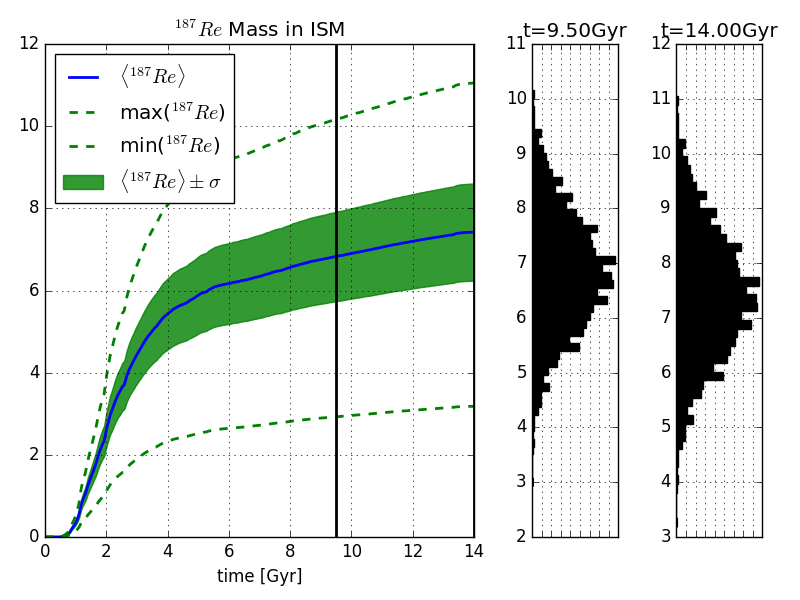
\includegraphics[width=\linewidth]{results/MCExperiment_revised_2/combined_plot_Re-187.png}
    \caption{\label{fig:MCExperiment-nodecay-re187}
      Total mass of \re{187} in the interstellar medium of the galaxy modelled by \omegamodel.
  }
  \end{subfigure}
  \begin{subfigure}{\subfigwidth}
    \centering
    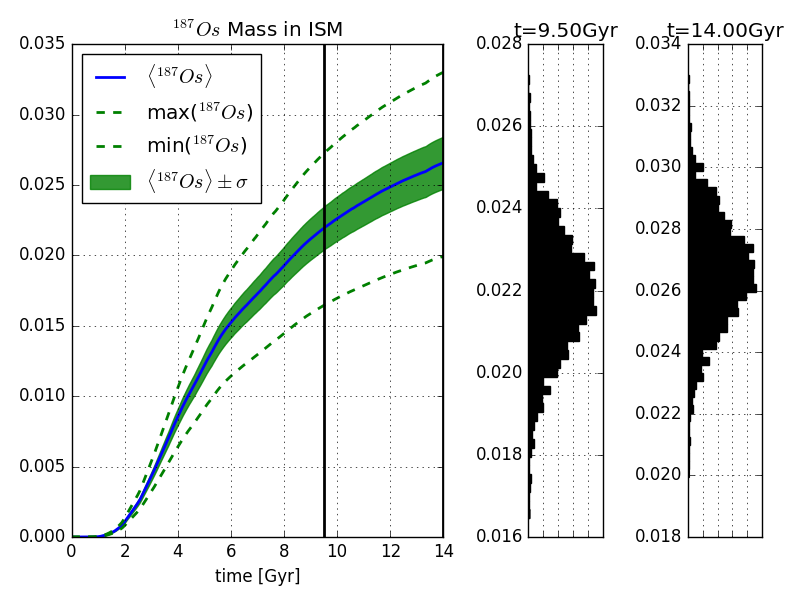
\includegraphics[width=\linewidth]{results/MCExperiment_revised_2/combined_plot_Os-187.png}
    \caption{\label{fig:MCExperiment-nodecay-os187}
      Total mass of \os{187} in the interstellar medium of the galaxy modelled by \omegamodel.
    }
  \end{subfigure}
  \begin{subfigure}{\figwidth}
    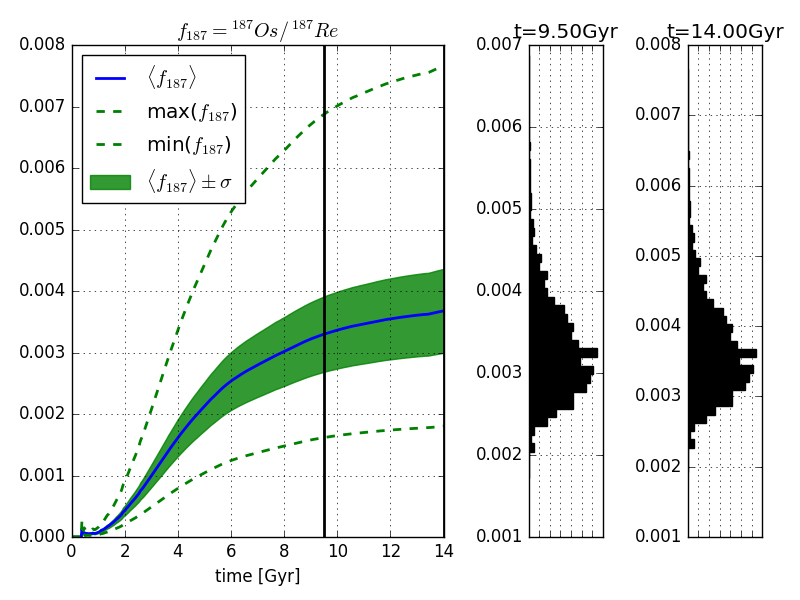
\includegraphics[width=\linewidth]{results/MCExperiment_revised_2/combined_plot_div.png}
    \caption{\label{fig:MCExperiment-nodecay-div}
      Fraction of \os{187} to \re{187} in the interstellar medium of the galaxy modelled by \omegamodel.
    }
  \end{subfigure}
  \caption[\expone\ before \betadecay]{\label{fig:MCExperiment-nodecay}
    The mass and mass fractions in the interstellar medium \textit{before} \betadecay is applied. Only nucleosynthesis/production from stellar sources is considered.

    The far left plot of all subfigures represent the timeevolution of the mass/mass-fraction in the interstellar medium, while the two right plots represent the uncertainty distribution at a given point in time. The points in time are 9.5 Gyrs (the formation of the solar system) and 14 Gyrs (current time). The points in time are also shown by black vertical lines in the far left plot.
  }
\end{figure}
\FloatBarrier %end of subsection

%add plots of Os-187, Re-187, Os-187/Re-187 for regular MCExperiment
\section{With \betadecay}
\label{sec:results-decay}
The cosmic clock fraction, $f_{187} = \frac{\os{187}}{\re{187}}$, is expected to increase with \betadecay, because amounts of \re{187} decays to \os{187} following the differential equation in section \ref{sec:betadecay}.
As outlined in the methods, a \betadecay\ calculation was applied to the data in postprocessing.
The resulting figures show a clear increase in cosmic clock fraction, as well as a significant decrease in uncertainty.
The decrease in uncertainty is discussed in chapter \ref{sec:conclusion}.

\begin{figure}
  \centering
  \begin{subfigure}{\subfigwidth}
    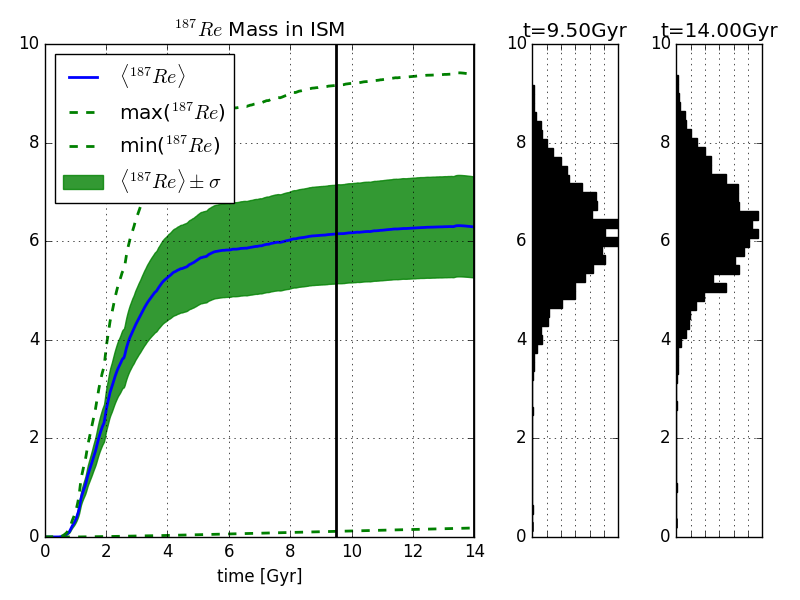
\includegraphics[width=\linewidth]{results/MCExperiment_revised_2/combined_plot_Re-187_decayed.png}
    \caption{\label{fig:MCExperiment-decay-re187}
      Total mass of \re{187} in the interstellar medium of the galaxy modelled by \omegamodel.
    }
  \end{subfigure}
  \begin{subfigure}{\subfigwidth}
    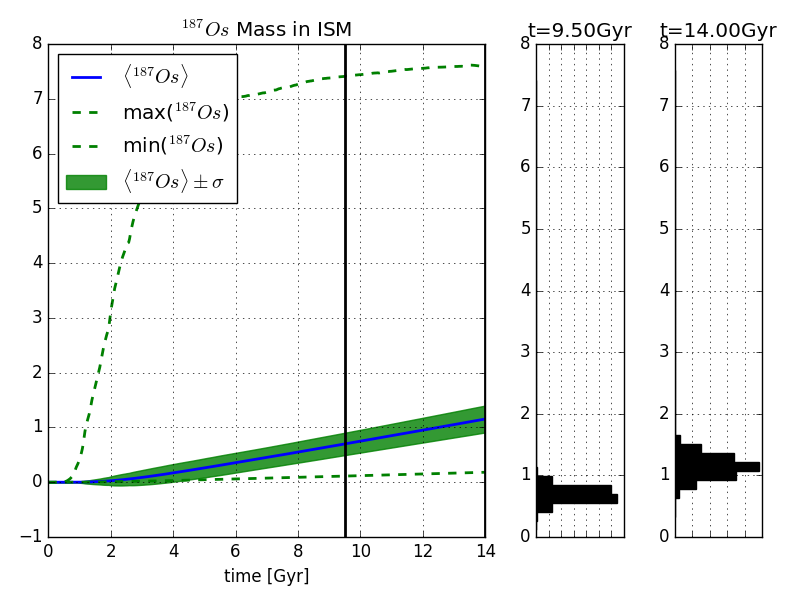
\includegraphics[width=\linewidth]{results/MCExperiment_revised_2/combined_plot_Os-187_decayed.png}
    \caption{\label{fig:MCExperiment-decay-os187}
      Total mass of \os{187} in the interstellar medium of the galaxy modelled by \omegamodel.
  }
  \end{subfigure}
  \begin{subfigure}{\figwidth}
    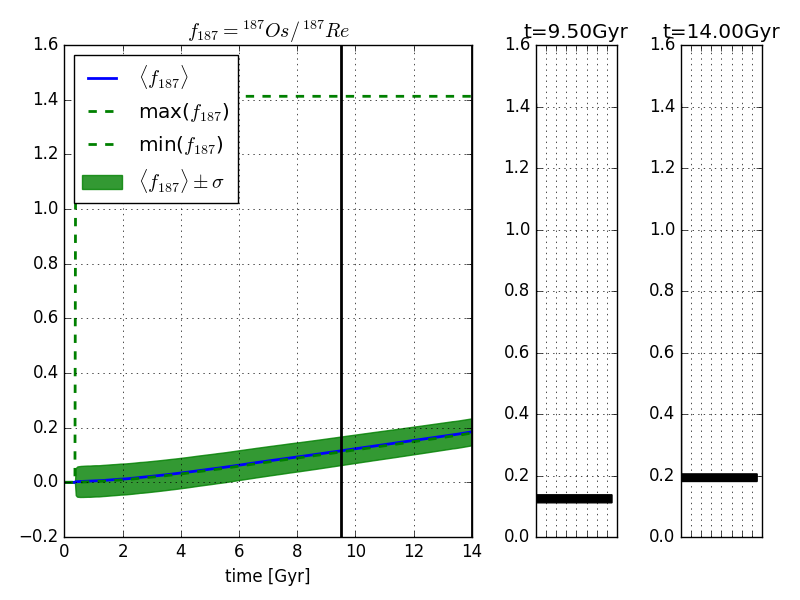
\includegraphics[width=\linewidth]{results/MCExperiment_revised_2/combined_plot_div_decayed.png}
    \caption{\label{fig:MCExperiment-decay-div}
      Fraction of \os{187} to \re{187} in the interstellar medium of the galaxy modelled by \omegamodel.
    }
  \end{subfigure}
  \caption[\expone\ after \betadecay]{\label{fig:MCExperiment-decay}
    The mass and mass fractions in the interstellar medium \textit{after} \betadecay is applied. Nucleosynthesis/production from stellar sources is considered as well as the radioactive decay from \re{187} to \os{187}.

    The far left plot of all subfigures represent the timeevolution of the mass/mass-fraction in the interstellar medium, while the two right plots represent the uncertainty distribution at a given point in time. The points in time are 9.5 Gyrs (the formation of the solar system) and 14 Gyrs (current time). The points in time are also shown by black vertical lines in the far left plot.
  }
\end{figure}
\FloatBarrier %end of subsection

\section{Removing negative isotope yields}
\label{sec:results-delmax}
Do to the gaussian distribution of input parameters and relatively large sample size (1500 model calculations) some isotope yields will be negative.
This is unphysical, and all negative yields will be set to zero in the calculation.
Forcing the stellar yield is the closest physical interpretation of a negative yield-value.

This effect leads to an overabundance of zero-yields which makes the distribution of input parameters un-gaussian.
Overabundances in parameter distributions of this scale leads to outliers in the results. Such outliers also greatly affect the standard deviation of the resulting distribution, see figure \ref{fig:MCExperiment-decay-div} for an example.
One possible solution to this is to take a gaussian distribution set it to zero below parameter-value zero and scale it to the integral (as is the norm for statistical distributions).
Applying this form of distribution numerically is beyond the capabilities of the writer. An alternate method is suggested. When the statistical distribution is found from the data, all models with a parameter-value of zero or lower $\hat{Y}_{\isotope{X}{Z}{A}} \leq 0 $, is ignored.

The resulting distributions are shown in figures \ref{fig:MCExperiment-delmax}, and the values for the distribution extracts (both with and without the effect of \betadecay) are shown in table \ref{tab:results-delmax}.

\newcommand\tworow[2]{\begin{tabular}{c}#1\\#2\end{tabular}}
\newcommand\midrow[2]{\raisebox{-#2}[#2]{#1}}
\newcommand\checkremaininglength{\leaders\vrule\vfill}
\begin{table}[h!]
  \begin{tabular}{|c|c|cc|}
    \hline {} & Postprocessed & \tworow{$t=9.5Gyr$}{\sos\ formation} & \tworow{$t=14Gyr$}{Now} \\
    \hline
    \hline \midrow{\re{187}}{2ex} & No \betadecay & $6.83 \pm 1.09$ \msol & $7.42 \pm 1.18$ \msol \\
    \cline{2-4} {\midrow{}{2ex}} & \betadecay applied & $6.16 \pm 0.98$ \msol & $6.3 \pm 1.00$ \msol \\
    \hline \midrow{\os{187}}{2ex} & No \betadecay & $0.02(19) \pm0.00(15)$ \msol & $0.02(66) \pm 0.00(18)$ \msol \\
    \cline{2-4} {\midrow{}{2ex}} & \betadecay applied & $0.70 \pm 0.11$ \msol & $1.15 \pm 0.18$ \msol \\
    \hline \midrow{$f_{187}$}{2ex} & No \betadecay & $0.00(33) \pm 0.00(06)$ & $0.00(37) \pm 0.00(07)$ \\
    \cline{2-4} {\midrow{}{2ex}} & \betadecay applied & $0.11(31) \pm 0.00(07)$ & $0.18(28) \pm 0.00(08)$ \\
    \hline
  \end{tabular}
  \caption[Mass-table at \sos\ formation and now for \expone]{\label{tab:results-delmax}
    Mean and standard deviation of mass and mass fraction in \omegamodel.
    Distributions with and without \betadecay were considered after calculations with negative yields were neglected.
    Values represent the distributions shown in figures \ref{fig:MCExperiment-delmax}, which are excerpts of the time-evolution graphs at the black vertical lines.
  }
\end{table}
%\checkremaininglength

%figure of zero-yield plots here
\begin{figure}
  \centering
  \begin{subfigure}{\subfigwidth}
    \includegraphics[width=\linewidth]{results/MCExperiment_revised_2_delmax/combined_plot_Re-187_decayed.png}
    \caption{ \label{fig:MCExperiment-delmax-re187}
      Mass of \re{187} in the interstellar medium of the galaxy modelled by \omegamodel.
    }
  \end{subfigure}
  \begin{subfigure}{\subfigwidth}
    \includegraphics[width=\linewidth]{results/MCExperiment_revised_2_delmax/combined_plot_Os-187_decayed.png}
    \caption{ \label{fig:MCExperiment-delmax-os187}
      Mass of \os{187} in the interstellar medium of the galaxy modelled by \omegamodel.
    }
  \end{subfigure}
  \begin{subfigure}{\figwidth}
    \includegraphics[width=\linewidth]{results/MCExperiment_revised_2_delmax/combined_plot_div_decayed_meteordata.png}
    \caption{ \label{fig:MCExperiment-delmax-div}
      Fraction of \os{187} to \re{187} in the interstellar medium of the galaxy modelled by \omegamodel.
    }
  \end{subfigure}
  \caption[\expone\ with \betadecay and removing negative isotope yields]{ \label{fig:MCExperiment-delmax}
    Same as figure \ref{fig:MCExperiment-decay} with datafiles corresponding to negative yields not considered in the distribution.
    
    The far left plot of all subfigures represent the timeevolution of the mass/mass-fraction in the interstellar medium, while the two right plots represent the uncertainty distribution at a given point in time (a distribution extract).
    The distribution extracts are taken at 9.5 Gyrs (the formation of the solar system) and 14 Gyrs (current time). The points in time are also shown by black vertical lines in the far left plot. \\
    The values for the mean and standard deviation (green line) in the distribution extracts can be found in table \ref{tab:results-delmax}.
    The green band represent meteordata calculated in appendix \ref{sec:calc-cosmo-chronology}.
  }
\end{figure}
\FloatBarrier %end of subsection

\section{Rate of nucleosynthetic events}
In \omegamodel, the nuclides in question are synthesized in stars and ejected into the interstellar medium through a limited list of events.
Asymptotic giant branch stars, massive stars that turn into type 2 supernvoae, type 1a supernovae, and binary neutron star mergers.
The merger of a black hole and a neutron star is not considered as it was not considered in the r-process postproduction of \eris\ (\mycite{shen15}).
In this seciton, the rate and cumulative number of these events are shown, see figures \ref{fig:MCExperiment-delmax-rate}.
The data was taken from \expone\ experiment, meaning that there is no uncertainty applied to the number and rate of events.
Extracts from the rates and cumulative numbers at the time of \sos\ formation and current time are shown in table \ref{tab:nucleosynthetic-events}

\begin{table}[h]
  \centering
  \begin{tabular}{|c|c|c|}
    \multicolumn{3}{c}{Binary neutron star mergers} \\ \hline
    time & rate & $\Sigma N$ \\ \hline 
    $14 Gyr$ & $0.201 Myr^{-1}$ & $114 \times 10^3$ \\ \hline 
    $9.49 Gyr$ & $3.75 Myr^{-1}$ & $101 \times 10^3$ \\ \hline
    \multicolumn{3}{c}{} \\
    \multicolumn{3}{c}{Type 1a supernovae} \\ \hline
    time & rate & $\Sigma N$ \\ \hline 
    $14 Gyr$ & $1.1 \times 10^{-44} Myr^{-1} \simeq 0 Myr^{-1}$ & $29.6 \times 10^{6}$ \\ \hline 
    $9.49 Gyr$ & $821 Myr^{-1}$ & $27.2 \times 10^{6}$ \\ \hline
    \multicolumn{3}{c}{} \\
    \multicolumn{3}{c}{type 2 supernovae} \\ \hline
    time & rate & $\Sigma N$ \\ \hline 
    $14 Gyr$ & $0 Myr^{-1}$ & $258 \times 10^{6}$ \\ \hline 
    $9.49 Gyr$ & $8.67 \times 10^{3} Myr^{-1}$ & $233 \times 10^{6}$ \\ \hline
  \end{tabular}
  \caption[Rates and numbers of nucleosynthetic events in \expone]{\label{tab:nucleosynthetic-events}
    Rates and total number of nucleosynthetic events for neuron star mergers, type 1a and 2 supernovae in \omegamodel.
    The time is taken at $\simeq$9.5 Gyrs (the formation of the solar system, and 14 Gyrs (now).
    Plots of the time evolution of nucleosynthetic events are shown in figures \ref{fig:MCExperiment-delmax-rate}.
  }
\end{table}

\begin{figure}
  \centering
  \begin{subfigure}{\subfigwidth}
    \includegraphics[width=\linewidth]{results/MCExperiment_revised_2_delmax/sn1a.png}
    \caption{ \label{fig:MCExperiment-delmax-sn1a}
      Type 1a supernovae.
    }
  \end{subfigure}
  \begin{subfigure}{\subfigwidth}
    \includegraphics[width=\linewidth]{results/MCExperiment_revised_2_delmax/sn2.png}
    \caption{ \label{fig:MCExperiment-delmax-sn2}
      Type 2 supernovae.
    }
  \end{subfigure}
  \begin{subfigure}{\figwidth}
    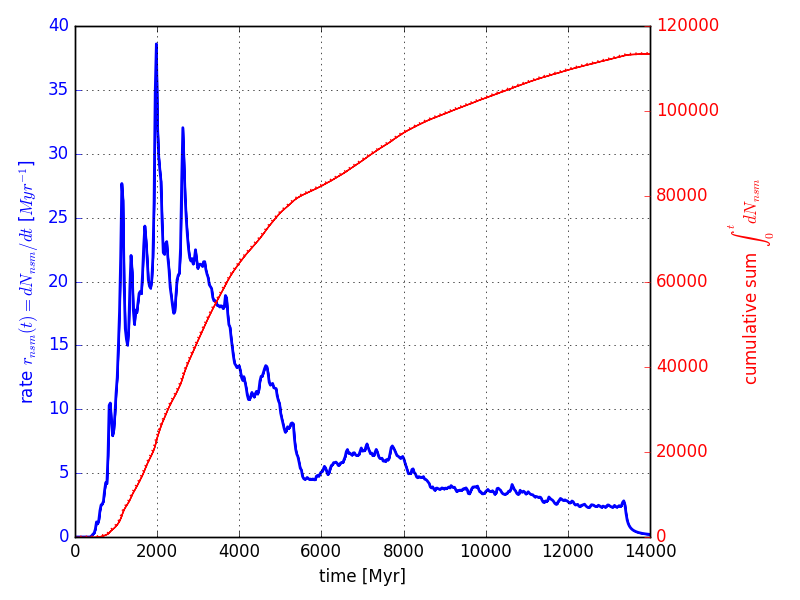
\includegraphics[width=\linewidth]{results/MCExperiment_revised_2_delmax/nsm.png}
    \caption{ \label{fig:MCExperiment-delmax-nsm}
      Binary neutron star mergers.
    }
  \end{subfigure}
  \caption[Rate of nucleosynthetic events]{ \label{fig:MCExperiment-delmax-rate}
    All plots show rate of nucleosynthetic events (blue), and cumulative sum of events (red)
    after \betadecay applied and negative isotope yields have been removed.
    The nucleosynthetic events are type 1a (\ref{fig:MCExperiment-delmax-sn1a}) and type 2 (\ref{fig:MCExperiment-delmax-sn2})
    supernovae, and binary neuron star mergers (\ref{fig:MCExperiment-delmax-nsm}).
    The rate of each event follows the star formation rate (see figure \ref{fig:sfr}) with a scale factor and delay time distribution.
  } 
\end{figure}
\FloatBarrier %end of subsection

\section{Comparing models}
With a numerical model for \os{187}/\re{187}, the data can be compared to other, analytical models.
All analytical models presented here are based on Claytons model for cosmochemical evolution of \os{187}/\re{187},
which assumes that the rate of events declines exponentially in time.
As can be seen in appendix \ref{sec:calc-cosmo-chronology} the actual number of events and the amount of \re{187} ejected from each is insignificant when calculating the fraction \os{187}$_c$/\re{187}. \os{187}$_c$ is the component of \os{187} from cosmoradiogenic decay from \re{187}.

The calculations in appendix \ref{sec:calc-cosmo-chronology} follow the analytical model of cosmochronology from \mycite{luck80}.
Like \mycite{luck80}, \mycite{shizuma05} also follows the analytical steps of \mycite{clayton64}.
A summary of models, parameters and references can be found in table \ref{tab:analytical-osre-models}.
\comment{\\ Possible error in figure, not uncertainty bands on shizuma and clayton suden models \\}

\begin{figure}[h]
  \centering
  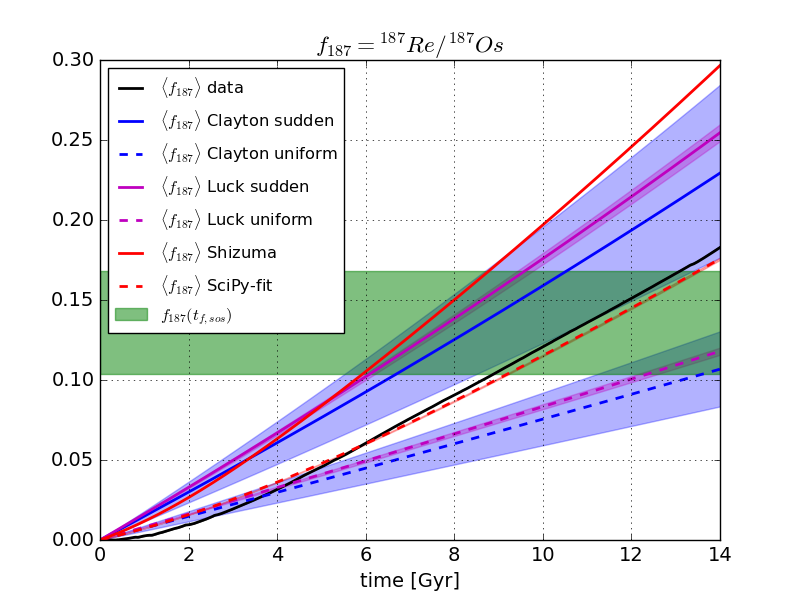
\includegraphics[width=\figwidth]{results/MCExperiment_revised_2_delmax/model_fitting.png}
  \caption[Analytical models for cosmochronology]{ \label{fig:osre-model-fitting}
    A comparison of the data from \omegamodel-experiment \expone (black), with the analytical models of Clayton (blue), Shizuma (green), and Luck (magenta) for comparison. \\
    The model from Shizuma is fitted to the data from \omegamodel, with the curvefit function in SciPy\footnote{\href{https://www.scipy.org/}{SciPy Homepage}} (seen in red).
    The green band represent meteordata calculated in appendix \ref{sec:calc-cosmo-chronology}.
  }
\end{figure}

\newgeometry{bottom=1cm}
\begin{landscape}
  \centering
  \begin{table}
    \centering
    \newcommand\leff{\lambda_{\tiny \beta}^{\textrm{\tiny eff}}}
    \newcommand\ditto[1]{\rule[0.5ex]{#1}{0.5pt}\raisebox{-0.5ex}{\textquotedbl}\rule[0.5ex]{#1}{0.5pt}}
    \newcommand\taure{\tau_{\scriptscriptstyle Re}}
    \newcommand\lamre{\lambda_{\scriptscriptstyle Re}}
    \begin{tabular}{|c|c|c|c|c|}
      \hline \small Model & \os{187}$_c$/\re{187} & $\lamre$ & $\lambda_{rncp}$ & Reference \\
      \hline \hline \small Clayton
      & $ \frac{\Lambda - \lambda}{\lambda} e^{\lambda t} \frac{1-e^{-\Lambda t}}{1-e^{-(\Lambda - \lambda) t}} - 1$
      & $\lambda = \frac{\ln 2}{\taure}$ & $\Lambda$ & \mycite{clayton64} \\
      \hline \small \tworow{Clayton}{Sudden synthesis}
      & $e^{\lambda t} - 1$
      & $\taure = 47 \pm 10 Gyr$ & $\Lambda \rightarrow \infty$ & \mycite{clayton64} \\
      \hline \small \tworow{Clayton}{Uniform synthesis}
      & $\frac{\lambda t}{1-e^{-\lambda t}} - 1$
      & \ditto{3em} & $\Lambda \rightarrow 0$ & \mycite{clayton64} \\
      \hline \small Luck &
      $\frac{\lamre/\beta (1-e^{-\beta t}) - (1-e^{-\lamre t})}{e^{-\beta t} - e^{-\lamre t}}$
      & $\lambda_{ \textrm{\tiny Re} } = \begin{array}{l} 1.62 \pm 0.08  \\ \times 10^{-11} yr^{-1} \end{array}$ & $\beta$ & \mycite{luck80} \\
      \hline \small \tworow{Luck}{Sudden synthesis}
      & \ditto{3em} & \ditto{3em}& $\beta = 10^{-6} yr^{-1}$ & \mycite{luck80} \\
      \hline \small \tworow{Luck}{Steady state}
      & \ditto{3em} & \ditto{3em} & $\beta = 10^{-12} yr^{-1}$ & \mycite{luck80} \\
      \hline \small Shizuma
      & $\frac{(1-e^{-\leff t}) - (1-e^{-\lambda t}) \leff / \lambda }{e^{-\leff t} - e^{-\lambda t}} $
      & $ \leff = \frac{ 1.2 \ln 2 }{\taure} = 2.00\times 10^{-11} [yr^{-1}]$ & $\lambda \in [0,2] Gyr^{-1}$ & \mycite{shizuma05} \\
      \hline \tworow{SciPy curvefit}{to \omegamodel-data} & \ditto{3em}
      & \tworow{$1.33\times 10^{-11} $}{$\pm 2.767\times 10^{-14}$} $[yr^{-1}]$
      & \tworow{$5.42\times 10^{-10} $}{$\pm 5.79\times 10^{-12}$} $[yr^{-1}]$ & \\
      \hline 
    \end{tabular}
    %% SciPy-fitting to data: (lambda_eff, lambda_rncp) = [  1.33343923e-11   5.42456343e-10] +/- [  2.76664355e-14   5.79209853e-12]/[  2.76664315e-14   5.79209788e-12]
    \caption[Analytical models for \os{187}$_c$/\re{187}]{ \label{tab:analytical-osre-models}
      Table with the analytical models in the literature, stemming from \mycite{clayton64}.
      Notation of parameters is attempted to be consistent with the articles they are taken from, not with eachother in the table.
      $\lambda_{\re{187}}$ is the decay constant of radioactive \re{187}.
      $\lambda_{rncp}$ is the decay constant of the rate of events for \textit{rapid neutron capture processes}.
      $\leff$ is the effective net \betadecay constant for \re{187} after thermal consitions of astration have been taken into account, equalt to 1.2 times \betadecay-constant of neutral \re{187}.
      Shizuma does not give any uncertainty for the halflife of \re{187}, and the boundaries of $\lambda$ are only found to be in good agreement with a Galctic age of 11-15 yrs.
      The basic model for Shizuma, Luck and Clayton are identical, even though they are written differently.
      Scipy curvefit is the parameters, with standard deviation, after fitting the model from \mycite{shizuma05} to the data produced in \omegamodel; \expone-experiment.
    }
  \end{table}
\end{landscape}
\restoregeometry
\FloatBarrier %end of subsection

\section{Consider high mass slope of initial mass function}
The initial mass function gives the distribution of masses for a stellar population.
Changing the high-mass slope of the mass function gives more stars with higher initial mass\footnote{Note that more stars with more mass does not change the total mass of gas turned to stars, but gives more high mass stars at the expense of fewer small mass stars.}.
High mass stars end their life as type 2 core collapse supernovae, with a significantly differentdistribution of nuclei.
It was found in \mycite{cote16a} that the slope of the initial mass function had the most significant impact on uncertainties in nucleosynthesis.

In a different set of \omegamodel-calculation, \exptwo, the slope of the initial mass function is varied as well, as described in the introduction to this chapter.
Figures \ref{fig:MCExperiment-imfslope} show the mass and massratio of \os{187} and \re{187}, the distribution at the formation of the oslar system and current time are imbedded as distribution extracts.
The mean and standard deviation of the distribution extract can be found in table \ref{tab:results-imf}, with and without \betadecay applied to the data.
From the distribution extracts in figures \ref{MCExperiment-imfslope} the distribution are clearly non-gaussian in nature, so the mean and standard deviation can be misleading.
It would be more meaningful to divide the distributions in two and calcualte the mean and standard deviation for the two separate distributions individually (especially for $f_{187}$ in figure \ref{MCExperiment-imfslope-div}).

\begin{table}[h]
  \begin{tabular}{|c|c|cc|}
    \hline {} & Postprocessed & \tworow{$t=9.5Gyr$}{\sos\ formation} & \tworow{$t=14Gyr$}{Now} \\
    \hline
    \hline \midrow{\re{187}}{2ex} & No \betadecay & $12.82 \pm 6.54$ \msol & $13.97 \pm 7.12$ \msol \\
    \cline{2-4} {\midrow{}{2ex}} & \betadecay applied & $11.57 \pm 5.91 $ \msol & $11.87 \pm 6.06$ \msol \\
    \hline \midrow{\os{187}}{2ex} & No \betadecay & $0.17 \pm 0.09$ \msol & $0.20 \pm 0.11$ \msol \\ 
    \cline{2-4} {\midrow{}{2ex}} & \betadecay applied & $1.41 \pm 0.64$ \msol & $2.29 \pm 1.08$ \msol \\
    \hline \midrow{$f_{187}$}{2ex} & No \betadecay & $0.01(80) \pm 0.01(70)$ & $0.01(98) \pm 0.01(89)$ \\
    \cline{2-4} {\midrow{}{2ex}} & \betadecay applied & $0.13 \pm 0.02$ & $0.20 \pm 0.02$ \\
    \hline
  \end{tabular}
  \caption[Mass-table as \sos\ formation and now for \exptwo]{\label{tab:results-imf}
    Mean and standard deviation of mass and mass fraction in \omegamodel; experiment \exptwo.
    Values represent the mean and standard deviations in the distribution extracts in figures \ref{MCExperiment-imf}.
  }
\end{table}

%add plots of Os-187, Re-187, Os-187/Re-187 for MCExperiment w/IMFslope
\begin{figure}
  \centering
  \begin{subfigure}{\subfigwidth}
    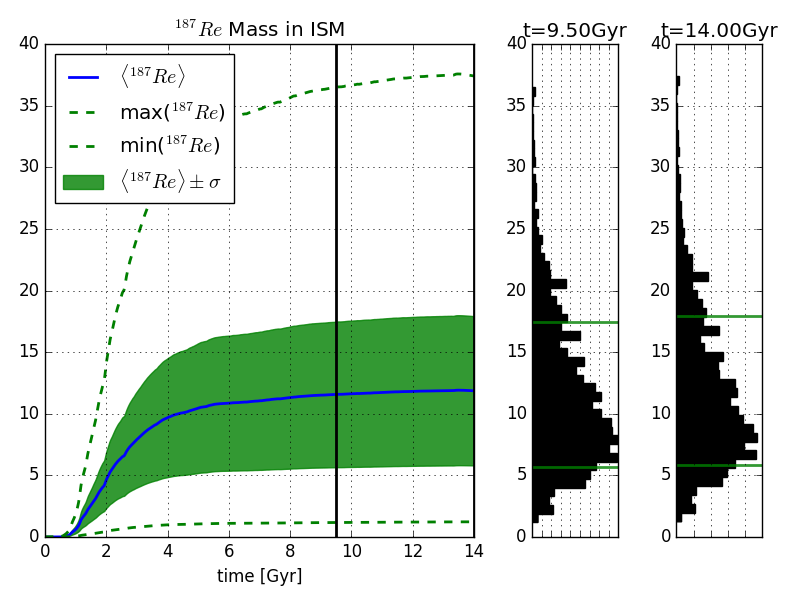
\includegraphics[width=\linewidth]{results/MCExperiment_revised_2_imfslope/combined_plot_Re-187_decayed.png}
    \caption{\label{fig:MCExperiment-imfslope-re187}
      Mass of \re{187} in the interstellar medium of the galaxy modelled by \omegamodel.
    }
  \end{subfigure}
  \begin{subfigure}{\subfigwidth}
    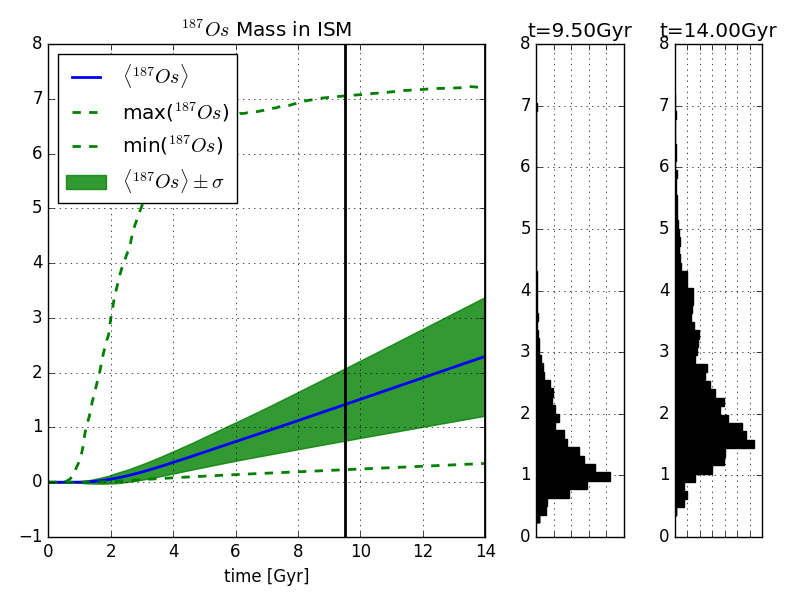
\includegraphics[width=\linewidth]{results/MCExperiment_revised_2_imfslope/combined_plot_Os-187_decayed.png}
    \caption{\label{fig:MCExperiment-imfslope-os187}
      Mass of \re{187} in the interstellar medium of the galaxy modelled by \omegamodel.
    }
  \end{subfigure}
  \begin{subfigure}{\figwidth}
    \includegraphics[width=\linewidth]{results/MCExperiment_revised_2_imfslope/combined_plot_div_decayed_meteordata.png}
    \caption{\label{fig:MCExperiment-imfslope-div}
      Fraction of \os{187} to \re{187} in the interstellar medium of the galaxy modelled by \omegamodel.
    }
  \end{subfigure}
  \caption[\exptwo\ after \betadecay and removing negative isotope yields]{\label{fig:MCExperiment-imfslope}
    The mass and mass fractions in the interstellar medium \textit{after} \betadecay is applied and uncertainty in the high mass slope of the initial mass function. Nucleosynthesis/production from stellar sources is considered as well as the radioactive decay from \re{187} to \os{187}. The amount of type II supernovae are also varied because the high mass slope of the initial mass function gives more massive stars, which in turn give more type II supernovae.

    The far left plot of all subfigures represent the timeevolution of the mass/mass-fraction in the interstellar medium, while the two right plots represent the uncertainty distribution at a given point in time. The points in time are 9.5 Gyrs (the formation of the solar system) and 14 Gyrs (current time). The points in time are also shown by black vertical lines in the far left plot.
  }
\end{figure}
\FloatBarrier %end of subsection

%(add plots of Os-187, Re-187, Os-187/Re-187 for MCExperiment w/NSMparameters)
\section{Consider events of binary neutron star mergers}
In the \expthree-experiment, the yields of stellar ejecta is varied as well as the slope of the initial mass function \textit{and} the physical parameters for neutron-star mergers.
These parameters are number of events, mass ejected per event, and the delay-time distribution of events.
Due to the lack of observational constraints it is hard to find quantifiable uncertainties for these parameters.
In order to estimate how the uncertainties of the neutron-star merger parameters affect the outcome a 10\% uncertianty is added to all parameters.

Figures \ref{MCExperiment-numnsm} show the mass and mass-ratio of \os{817} and \re{187}, while figures \ref{MCExperiment-numnsm-rate} show the rate and cumulative numbers of nucleosynthetic events in the \expthree-experiment.

\comment{Considering cut this section out, because the results look wrong and I don't know why. Uncertainty of rates vary by factors, while mass fraction is barely affected.}

\begin{figure}[h]
  \centering
  \begin{subfigure}{\subfigwidth}
    \includegraphics[width=\linewidth]{results/MCExperiment_revised_2_numnsm/combined_plot_Re-187_decayed.png}
    \caption{\label{fig:MCExperiment-numnsm-re187}
      Mass of \re{187} in the interstellar medium of the galaxy modelled by \omegamodel.
    }
  \end{subfigure}
  \begin{subfigure}{\subfigwidth}
    \includegraphics[width=\linewidth]{results/MCExperiment_revised_2_numnsm/combined_plot_Os-187_decayed.png}
    \caption{\label{fig:MCExperiment-numnsm-os187}
      Mass of \re{187} in the interstellar medium of the galaxy modelled by \omegamodel.
    }
  \end{subfigure}
  \begin{subfigure}{\figwidth}
    \includegraphics[width=\linewidth]{results/MCExperiment_revised_2_numnsm/combined_plot_div_decayed_meteordata.png}
    \caption{\label{fig:MCExperiment-numnsm-div}
      Fraction of \os{187} to \re{187} in the interstellar medium of the galaxy modelled by \omegamodel.
    }
  \end{subfigure}
  \caption[\expthree\ after \betadecay and removing negative isotope yields]{\label{fig:MCExperiment-numnsm}
    The mass and mass fractions in the interstellar medium \textit{after} \betadecay is applied to experiment \expthree. Nucleosynthesis/production from stellar sources is considered as well as the radioactive decay from \re{187} to \os{187}.

    The far left plot of all subfigures represent the timeevolution of the mass/mass-fraction in the interstellar medium, while the two right plots represent the uncertainty distribution at a given point in time. The points in time are 9.5 Gyrs (the formation of the solar system) and 14 Gyrs (current time). The points in time are also shown by black vertical lines in the far left plot.
  }
\end{figure}

\begin{figure}[h]
  \centering
  \begin{subfigure}{\subfigwidth}
    \includegraphics[width=\linewidth]{results/MCExperiment_revised_2_numnsm/sn1a.png}
    \caption{ \label{fig:MCExperiment-numnsm-sn1a}
      Type 1a supernovae.
    }
  \end{subfigure}
  \begin{subfigure}{\subfigwidth}
    \includegraphics[width=\linewidth]{results/MCExperiment_revised_2_numnsm/sn2.png}
    \caption{ \label{fig:MCExperiment-numnsm-sn2}
      Type 2 supernovae.
    }
  \end{subfigure}
  \begin{subfigure}{\figwidth}
    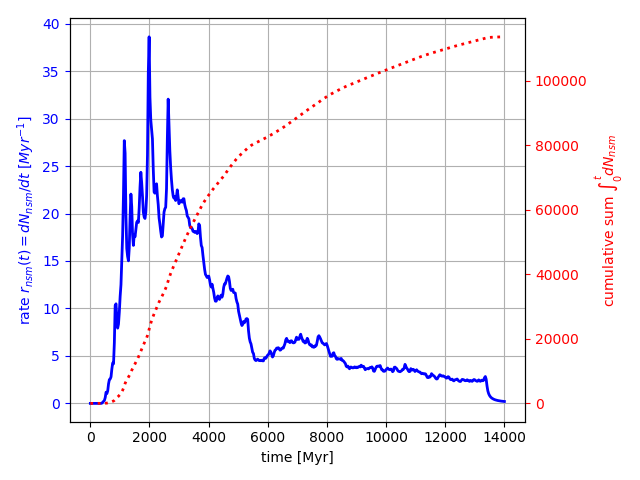
\includegraphics[width=\linewidth]{results/MCExperiment_revised_2_numnsm/nsm.png}
    \caption{ \label{fig:MCExperiment-numnsm-nsm}
      Binary neutron star mergers.
    }
  \end{subfigure}
  \caption[Rate of nucleosynthetic events \expthree]{ \label{fig:MCExperiment-numnsm-rate}
    All plots show rate of nucleosynthetic events (blue), and cumulative sum of events (red) for \expthree-experiment
    after \betadecay applied and negative isotope yields have been removed.
    The nucleosynthetic events are type 1a (\ref{fig:MCExperiment-numnsm-sn1a}) and type 2 (\ref{fig:MCExperiment-numnsm-sn2})
    supernovae, and binary neuron star mergers (\ref{fig:MCExperiment-numnsm-nsm}).
    The rate of each event follows the star formation rate (see figure \ref{fig:sfr}) with a scale factor and delay time distribution.
    The uncertainties come from a 10\% gaussian uncertainty in number of neutron star mergers, the delay-time distribution of neutron star mergers, and the uncertainty of the slope of the initial mass function.
  } 
\end{figure}
\FloatBarrier %end of subsection

